\documentclass[letterpaper, 10pt]{article}

%---- packages----------------------------%
\usepackage{geometry}
\usepackage{titling}
\usepackage{hyperref}
\usepackage{ulem}
\usepackage{booktabs}
\usepackage{siunitx}
\usepackage{graphicx} % http://ftp.math.purdue.edu/mirrors/ctan.org/macros/latex/required/graphics/grfguide.pdf
\usepackage{amsmath}
\usepackage{siunitx}
\usepackage{natbib}
%----------------------------------------------%

\begin{document}

\setlength{\droptitle}{-8em} 
\title{\Large\textbf{Trait-based Simulation of Microbiomes across a Climate Gradient}\vspace{-0em}}
\author{\normalsize\textbf{Bin Wang\textsuperscript{1}, Steven D. Allison\textsuperscript{1,2}}\vspace{1em} \\
\textsuperscript{1}Ecology and Evolutionary Biology, \textsuperscript{2}Earth System Science \\
University of California Irvine\vspace{0em} \\
Email: bwang7@uci.edu} 
%\date{\normalsize August, 2020\vspace{0em}}
\maketitle

This document serves to detail the parameterization of DEMENTpy across the Southern California
climate gradient, and supplement the main manuscript with model formulation, supporting text and results.

\section{DEMENTpy}

\subsection{Dispersal}
Dispersal is a key process in microbiome assembly and functioning. DEMENTpy deals with
dispersal explicitly with a few assumptions on environmental factors controlling dispersal rate ($R_{d}$),
which follows:
\begin{equation}
  R_{d} = ?? 
\end{equation}


\section{Climate gradient and derivation of forcings}
This document details the preparation for DEMENTpy inputs at each of the five sites simulated across the climate
gradient (\textbf{Figure 1}). In detail, inputs including water potential, soil temperature, and litter chemistry were
processed and derived. Water potential was derived from precipitation via an intermediate step of converting the
precipitation data. Python code (in the format of Jupyter Notebook, i.e., .ipynb) underlying all of the processing is
accessible at a GitHub Repo (\url{https://github.com/bioatmosphere/microbiome-climate-gradient.git}). With step-by
step demonstrations, those readers who have a keen interest are supposed to be able to easily reproduce these
preparations.

% figure of the location of the five sites
\begin{figure}[h]
\centering
  %\begin{center}
      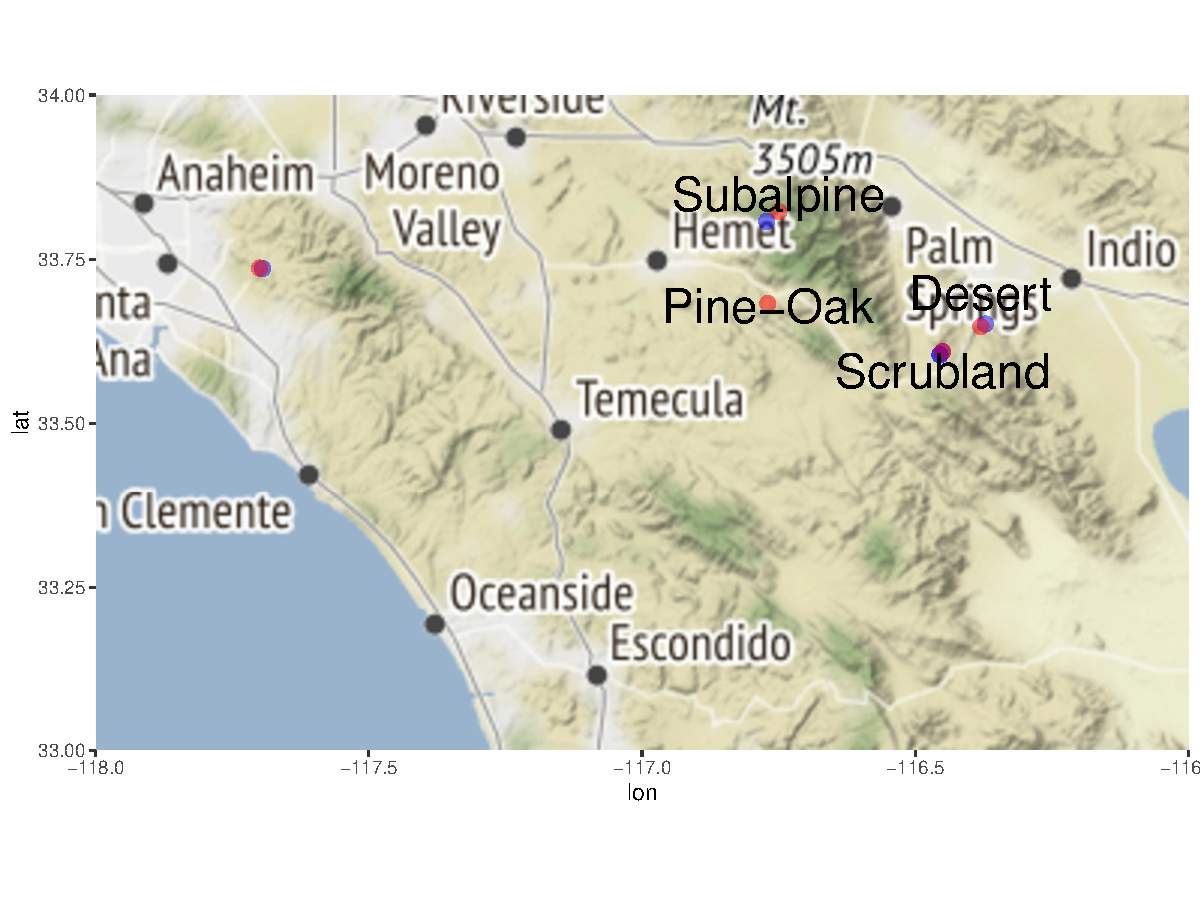
\includegraphics[scale=0.5]{site_location_v1.pdf}
      \caption{Location of the five sites across the gradient.}
      \label{fig: figure 1}
  %\end{center}
\end{figure}

\subsection{\large Ecosystems across the Southern California climate gradient}

% table of the basic features of the five sites 
\begin{table}[h!]
  \begin{center}
    \caption{Five sites across the climate gradient.}
    \label{tab: table1}
    \begin{tabular}{lccc}
      \toprule % <-- Toprule here
      \textbf{Site} & \textbf{Latitude} & \textbf{Longitude} & \textbf{Elevation}\\
      %$\alpha$ & $\beta$ & $\gamma$ \\
      \midrule % <-- Midrule here
      Desert       & 33.648 & -116.38 & 275\\
      Scrubland & 33.610 & -116.45 & 1280\\
      Grassland & 33.737 & -117.70 & 470\\
      Pine-Oak  & 33.683 & -116.77  & 1710\\
      Subalpine & 33.823 & -116.75  & 2250\\
      \bottomrule % <-- Bottomrule here
    \end{tabular}
  \end{center}
\end{table}

All five sites (\textbf{Table 1}) are located on granitic parent material and experience Mediterranean precipitation
patterns (cool, wet winters; hot, dry summers). This climate gradient covers a temperature range from ... to...



\subsection{\large Climate Forcing}

\subsubsection{Precipitation}
Longterm daily precipitation data were accessed from various sources for the five sites:

\textbf{Desert}: daily precipitation data from Boyd Deep Canyon California accessible at \url{https://wrcc.dri.edu/cgi-bin/rawMAIN.pl?caucde}

\textbf{Scrubland}: daily precipitation data from Burns Pinon Ridge Reserve California accessible at \url{https://wrcc.dri.edu/cgi-bin/rawMAIN.pl?caucbu}

\textbf{Grassland}:

\textbf{Pine-Oak}: daily precipitation data from James Reserve Station, California available at \url{https://wrcc.dri.edu/cgi-bin/rawMAIN.pl?caucja}

\textbf{Subalpine}: Since there was no station directly next to the Subalpine site, the precipitation at this site is likely
underestimated. In Glassman et al. (2019), precipitation was averaged from three NOAA weather stations with
heated gauges accounting for snow (USC00045091; US1CARV0002; and USC00044211): \url{https:/
www.ncdc.noaa.gov/cdo-web/datasets#GHCND}. Instead, daily precipitation data from station Mt. San Jacinto
California (\url{https://raws.dri.edu/cgi-bin/rawMAIN.pl?caCMSJ}) was accessed.

\subsubsection{Dead Fuel Moisture}

Dead Fuel moisture \url{https://www.wfas.net/index.php/dead-fuel-moisture-moisture--drought-38}


\subsubsection{Water Potential ($\psi$)}
As there are no direct measurements of water potential ($\psi$; unit: MPa) across the gradient, an approximation
was applied. This approximation is based on the only available, indirectly derived water potential data at the
grassland site. With available measurements of water content ($\theta$; unit: g H\textsubscript{2}O
g\textsuperscript{-1} wood), daily water potential was derived by \citet{allison2017consequences} at the grassland
site for a record of $?????$. This derivation of water potential followed a conversion from water content to water
potential as per the equation [\citet{dix1985changes}, referenced in \citet{allison2017consequences}]:

\begin{equation}
  \psi_{grassland} = -10^{0.118-0.114\log_{10} \theta}
\end{equation}

Water potential of all the other four sites ($\psi_{site}$) were then derived by linearly scaling grassland site water
potential ($\psi_{grassland}$) based on the Total Annual Precipitation(\textbf{TAP}; unit: mm) at each site following:

\begin{equation}
  \psi_{site} = \frac{TAP_{site}}{TAP_{grassland}} \psi_{grassland}
\end{equation}

One condition that makes this approximate scaling legitimate is the same Mediterranean precipitation patterns
across the climate gradient (cool, wet winters and hot, dry summers).


\subsubsection{Temperature (\SI{}{\celsius})}
DEMENTpy is conceived using litter temperature at a daily resolution in principle. In practice, soil temperature is
used instead to approximate the litter temperature. Soil temperature data at a sub-daily time step across the gradient
at each of five sites were measured. Details with regards to the measurement method, pre-, and post-processing are
documented in \citet{glassman2018decomposition}. These data are openly accesible at \url{https://github.com
stevenallison/UCIClimateExperiment/tree/master/updatednames}. From these field measurements, daily soil
temperature was derived by averaging all measurements in each day. A step-by-step demonstration of this derivation
is presented in the Jupyter Notebook \textbf{\texttt{soil\_temperature.ipynb}}.


\subsection{\large Litter Chemistry and Input}
DEMENTpy requires substrate-specific inputs in terms of C, N, and P (\textbf{Table xx}). \textbf{Phospholipids}
(i.e.,OrgP1 in the model) are a key component of all cell membranes(\url{https://en.wikipedia.org/wiki/Phospholipid}).
Though compound-specific stoichiometry is clear for determining concentration by element, substrate-specific
concentration (($Sub_i$); unit: mg cm\textsuperscript{-3}) needs to be determined. This derivation followed:
\begin{equation}
  Sub_{s,i} = Fraction_{s,i} Total_s 
\end{equation}
where $s$ is one of the five sites, $i$ is one of the 10 substrates, $Fraction_{s,i}$ is the percentage of substrate $i$
in site $s$, and $Total_s$ is the total concentration of initial substrates (C+N+P) in site $s$.  $Fraction$ was
informed by field measurements of litter chemistry at each site as presented in \citet{baker2017extracellular}. $Total$
was approximated by NPP at each site. As per the observation by \citet{baker2017extracellular}, standing litter pools
are largest in the grassland and pine-oak site, reduced in the subalpine site, significantly reduced in the scrubland
site, and negligible in the desert site. A detailed script implementing these processes is presented in the Jupyter
Notebook \textbf{\texttt{litter\_chemistry\_v1.ipynb}}.


%\newpage
\bibliographystyle{authordate1}
\bibliography{references}

\end{document}